\documentclass{article}
\usepackage{graphicx}
\usepackage{geometry}
\usepackage{minted}
\geometry{left=3.0cm,right=3.0cm,top=3.0cm,bottom=3.0cm}
\renewcommand{\thesection}{Problem \arabic{section}.}
\title{VE270 Homework 5}
\author{Liu Yihao 515370910207}
\date{}

\begin{document}
\maketitle

\section{}
\noindent Verilog Code:
\inputminted{verilog}{Q1.v}
\noindent Simulation Result:
\begin{center}
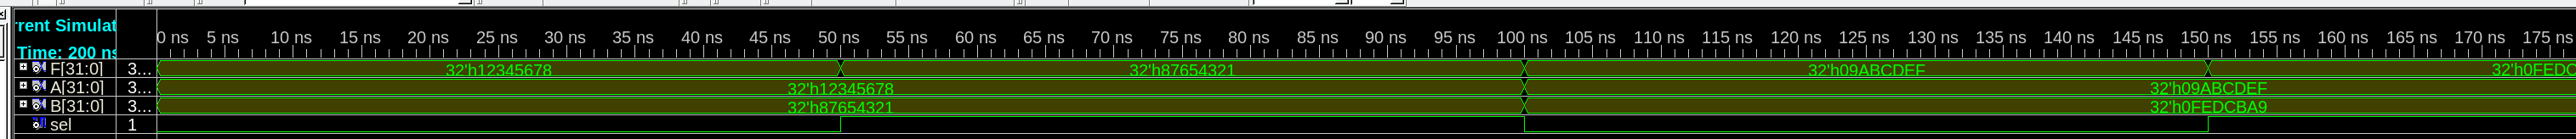
\includegraphics[width=0.95\linewidth]{Q1.png}
\end{center}

\newpage
\section{}
\noindent Verilog Code:
\inputminted{verilog}{Q2.v}
\noindent Simulation Result:
\begin{center}
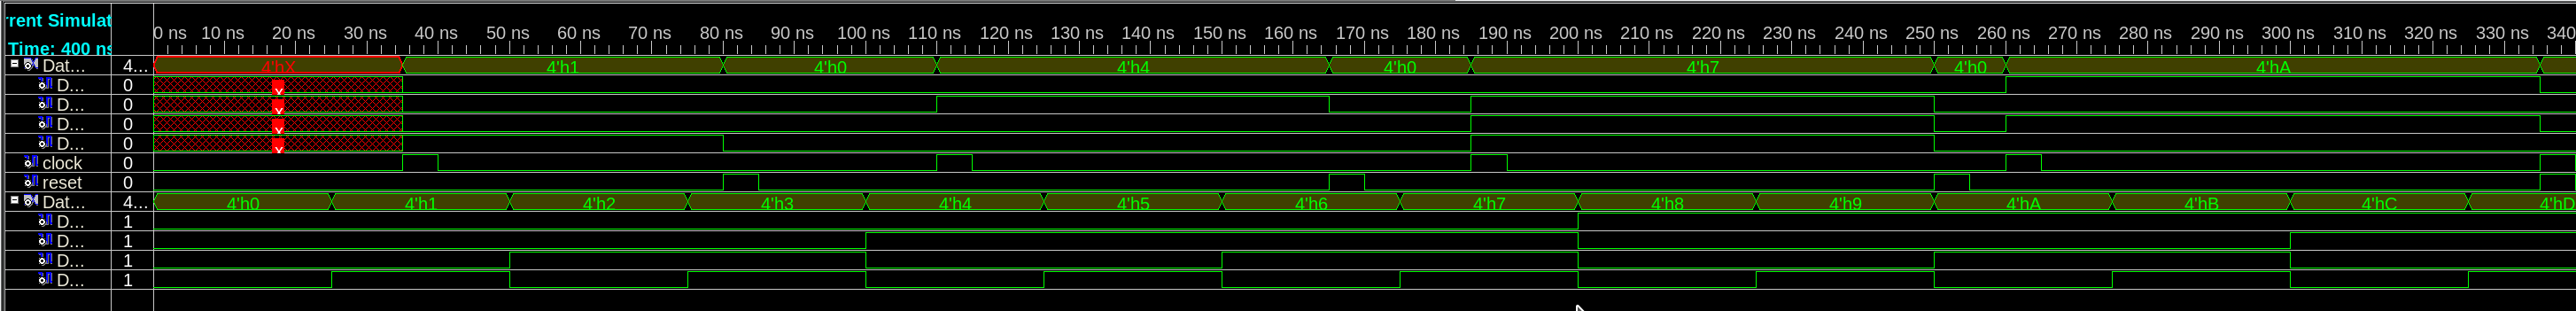
\includegraphics[width=0.95\linewidth]{Q2.png}
\end{center}

\newpage
\section{}
\noindent Verilog Code:
\inputminted{verilog}{Q3.v}
\noindent Simulation Result:
\begin{center}
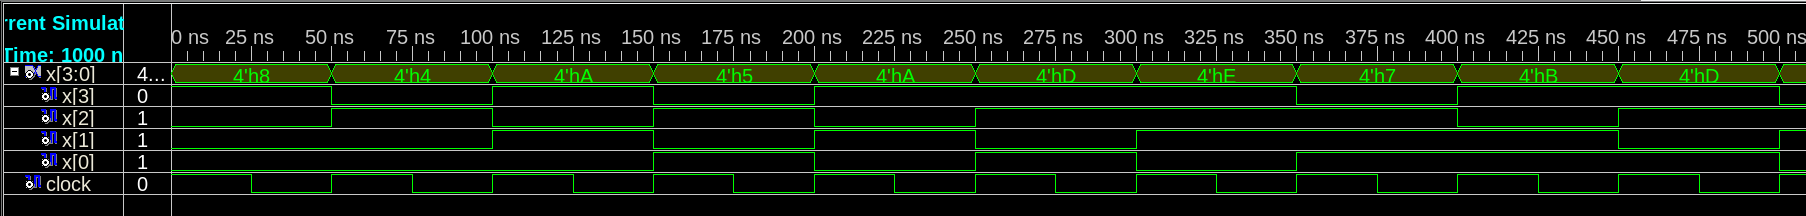
\includegraphics[width=0.95\linewidth]{Q3.png}
\end{center}

\newpage
\section{}
\noindent Verilog Code:
\inputminted{verilog}{Q4.v}
\noindent Simulation Result:
\begin{center}
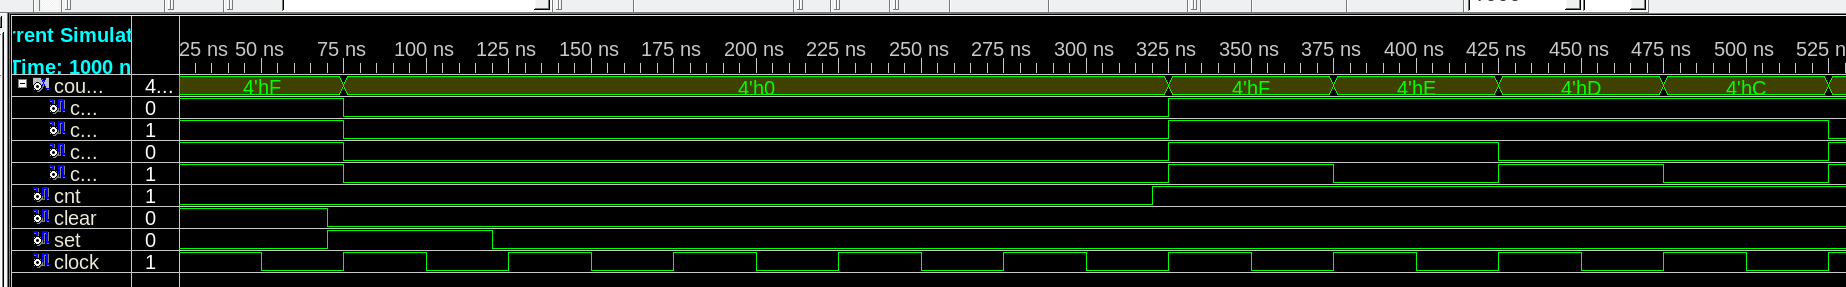
\includegraphics[width=0.95\linewidth]{Q4.png}
\end{center}

\newpage
\section{}
\noindent Verilog Code:
\inputminted{verilog}{Q5.v}
\noindent Simulation Result:
\begin{center}
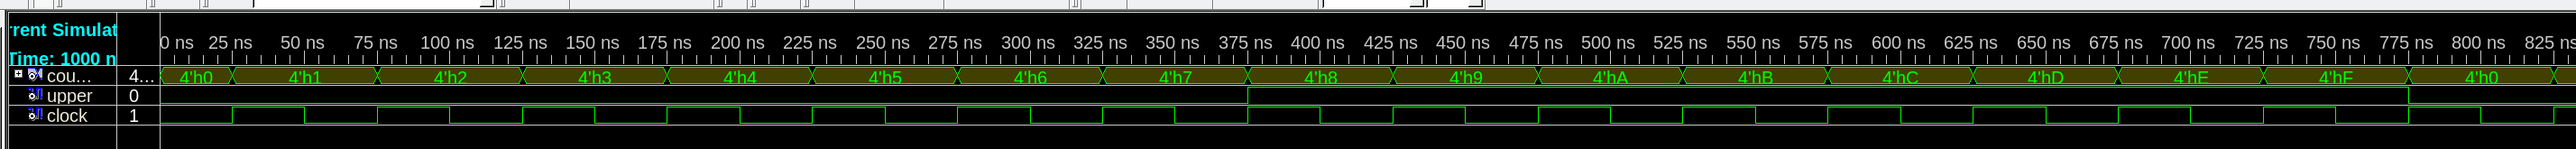
\includegraphics[width=0.95\linewidth]{Q5.png}
\end{center}



\end{document} 
